\documentclass[12pt,a4paper]{article}
\usepackage{fancyhdr}
\usepackage{fontspec}
\usepackage{amsmath}
\usepackage{amssymb}
\usepackage{bm}
\usepackage{tikz}
\usepackage{pstricks-add}
\setmainfont{Microsoft YaHei}
\pagestyle{fancy}


\begin{document}

\fancyfoot[C]{by chinasjtu@msn.com }

\newcommand{\nl}{\newline}

\newcommand{\ntinf}{\lim\limits_{n \to \infty}}
\newcommand{\xtinf}{\lim\limits_{x \to \infty}}

\newcommand{\Atinf}{\lim\limits_{A \to \infty}}
\newcommand{\Rtinf}{\lim\limits_{R \to \infty}}

\newcommand{\ntx}[1]{\lim\limits_{n \to #1}}
\newcommand{\xtx}[1]{\lim\limits_{x \to #1}}
\newcommand{\ttx}[1]{\lim\limits_{t \to #1}} 
\newcommand{\ktx}[1]{\lim\limits_{k \to #1}} 
\newcommand{\dxtx}[1]{\lim\limits_{\Delta x \to #1}}

\newcommand{\jfab}{\int_{a}^{b}}
\newcommand{\jf}[2]{\int_{#1}^{#2}}

\newcommand{\nsum}[2]{\sum\limits_{n=#1}^{#2}}
\newcommand{\isum}[2]{\sum\limits_{i=#1}^{#2}}
\newcommand{\ksum}[2]{\sum\limits_{k=#1}^{#2}}

\newcommand{\nsuminf} {\nsum{1}{\infty}}
\newcommand{\ksuminf} {\ksum{1}{\infty}}
\newcommand{\isuminf} {\isum{1}{\infty}}



$\nl$

\begin{center} 第二章 极限与连续初论  \end{center}
$\nl$
$\S2.1.数列极限$
$\nl$
一.概念

1)定义p.29. $\ntinf x_n=a 就是 \exists a \in R , \forall \varepsilon > 0, \exists N \in \bm{N}:|x_n-a|<\varepsilon, \forall n>N $
$\nl$
ex.①.

$$\lim_{n \to 0} \frac{1}{(1+\frac{1}{\sqrt{n}})^n}=0$$

因为$(1+a)^n \ge 1+na$

故$\frac{1}{(1+\frac{1}{\sqrt{n}})^n} \le \frac{1}{1+\frac{n}{\sqrt n}} = \frac {1}{1+\sqrt n}< \frac{1}{\sqrt n}$

对于$\forall \varepsilon >0 要使\frac{1}{\sqrt n}<\epsilon,即n> \frac{1}{\varepsilon ^ 2},取N=[\frac {1}{\varepsilon ^ 2}]+1$

$\nl$
ex.②.

$$\lim_{n \to \infty} q^n = 0 (0<q<1)$$

$设\frac{1}{q}= 1+\alpha (\alpha > 0)$

$|q^n-0|= \frac{1}{(1+\alpha)^n} \le \frac{1}{1+n\alpha} < \frac{1}{n\alpha}$

对于$\forall \varepsilon > 0, 取n>\frac{1}{\alpha \varepsilon} .......$

$\nl$
$$\lim_{n \to \infty}n^{\frac{1}{n}}=1,当n\ge 2,令n^{\frac{1}{n}}-1=h_n>0即证\lim_{n \to \infty}h_n=0$$

$由定义n=(1+h_n)^n=1+n\cdot h_n+\frac{n(n-1)}{2!}{h_n}^2+......+{h_n}^n>\frac{n(n-1)}{2}{h_n}^2$

$所以0<h_n<\sqrt{\frac{2}{n-1}} (n \ge 2)$

$对\forall \varepsilon > 0 由\sqrt{\frac{2}{n-1}} < \varepsilon 得 n>\frac{2}{\varepsilon ^2}+1$

$取N=max[1,[\frac{2}{\varepsilon ^ 2}]+1]$

$\nl$
(2)极限$$\lim_{n \to \infty}x_n=a等价命题$$

$1^\circ \forall \varepsilon>0 ,\exists N \in \bm{N}:|x_n-a|<\varepsilon,\forall n>N$

$2^\circ \forall \varepsilon(0<\varepsilon<1) ,\exists N \in \bm{N}:|x_n-a|<\varepsilon,\forall n>N$

$3^\circ \forall \varepsilon>0 ,\exists N \in \bm{N}:|x_n-a|<m\varepsilon,\forall n>N(m>0为常数)$

$4^\circ \forall \varepsilon>0 ,只有有限个x_n满足|x_n-a|\ge\varepsilon$

$\nl$

$2^\circ \Rightarrow 1^\circ,\forall \epsilon>0,\exists \epsilon'(0<\epsilon'<1):\epsilon'<\epsilon,由条件2^\circ,\exists N \in \bm{N}:|x_n-a|<\epsilon'<\epsilon,\forall n>N$

$3^\circ \Rightarrow 1^\circ,\forall \epsilon>0,\exists \epsilon'=\frac{\epsilon}{m}>0,由3^\circ,\exists N \in \bm{N},|x_n-a|<m\epsilon'=\epsilon,\forall n>N$

$\\$

二.收敛数列定理

唯一性,若{$x_n$}收敛,则极限值必唯一

设$$\lim_{x \to \infty}x_n=a, \lim_{x \to \infty}x_n=b(b>a)$$

令$\varepsilon_0=\frac{1}{2}(b-a),则a-\varepsilon_0<x_n<a+\varepsilon_0,\forall n>N_1$

$b-\varepsilon_0<x_n<b+\varepsilon_0,\forall n>N_2$

$取N=max(N_1,N_2)$

$x_n>b-\varepsilon_0=\frac{a+b}{2}=a+\varepsilon_0>x_n$,矛盾

$\nl$
定义2,若
$\exists M>0:|x_n|\le M,\forall n \in \bm{N}称{x_n}有界$

$\nl$
定理2,收敛数列必有界

$\nl$
定理3(保号性),若
$$\lim_{n \to \infty}x_n=a>0,必\exists N \in \bm{N}:x_n>0,\forall n > N$$

推论1,若
$$\lim_{n \to \infty}x_n=a>b,必存在N\in \bm{N}:x_n>b,\forall n>N$$

推论2,若
$$\lim_{n \to \infty}x_n=a,\lim_{n \to \infty}y_n=b,a>b,必存在N\in \bm{N}:x_n>y_n,\forall n>N$$

$\nl$
定理4,四则运算法则,前提(极限存在,有限次运算)

$\nl$
$子列概念,P94,若\ntinf x_n=a,\forall \{x{_nk}\} \subset \{x_n\},\ntinf x_{nk}=a$

若$$\lim_{n \to \infty}x_n=a,\forall \left\{ x_{nk} \right\} \subset \left\{ x_n \right\},\lim_{n \to \infty}x_{nk}=a$$

命题,数列收敛充要条件:奇偶子列均收敛于同一极限

$\nl$
五.数列收敛的条件
$\nl$
(1)迫敛性定理

定理6.设$$\lim_{n \to \infty}y_n=\lim_{n \to \infty}z_n=a,且对\forall n \in N,y_n \le x_n \le z_n,则有$$

$$\lim_{n \to \infty}x_n=a$$

例$(n+1)^\alpha - n^\alpha (0<\alpha<1)=n^\alpha (1+\frac{1}{n})^\alpha - n^\alpha<n^\alpha(1+\frac{1}{n}-1)=\frac{1}{n^{1-\alpha}}$
$故\ntinf (n+1)^\alpha - n^\alpha = 0$

$\nl$
(2)确界原理(P96确界定义)

该问题证明应利用定义

ex1. $inf(x_n)+inf(y_n)\le inf(x_n+y_n) \le
\begin{Bmatrix} inf(x_n)+sup(y_n) \\ sup(x_n)+inf(y_n) \end{Bmatrix} \le sup(x_n+y_n) \le sup(x_n)+sup(y_n)
$

$inf(x_n+y_n) \le x_n+yn \le x_n+sup(y_n)$

$故有设p=inf(x_n+y_n)-sup(y_n) \le x_n$

$所以p为x_n一个下界,则p \le inf(x_n)$

$所以inf(x_n+y_n) \le inf(x_n)+sup(y_n)$

$\nl$
(3)单调有界定理 p43 p100

$$x_{n+1}=1+\frac{x_n}{1+x_n},\lim_{n \to \infty}x_{n+1}=1+\frac{\lim\limits_{n \to \infty}x_n}{1+\lim\limits_{n \to \infty}x_n}=\lim_{n \to \infty}x_n$$

$$\lim_{n \to \infty}x_n=\frac{1+\sqrt 5}{2}$$

$\nl$

$x_{n+1}=\frac{1}{3}(2x_n+\frac{a}{x_n^2})\ge \sqrt[3]{a}$

$x_{n+1}=\frac{2x_n^3+a}{3x_n^2} \le \frac{2x_n^3+x_n^3}{3x_n^2}=x_n$

$\nl$
例题:$设a>0, x_1=a^{\frac{1}{p}} (p \in N), x_{n+1}=\frac{p-1}{p}x_n+\frac{a}{p}x_n^{1-p}$

$$假设x_n \ge \sqrt[p]{a} \to  x_{n+1} \le x_n \to \lim_{n \to \infty}x_n = \sqrt[p]{a}$$

$\nl$
(4)柯西收敛原理 p104,

$等价命题, \forall \varepsilon>0, \exists N \in \bm N: |x_{n+p}-x_n|< \varepsilon , \forall n>N, \forall p \in \bm N$

结果须与p无关

$\\$
习题课(数列极限)

一、概念

(1)与$\lim\limits_{n \to \infty}x_n=a等价?$

$\exists N \in \bm N, \forall \varepsilon >0:|x_n-a|<\varepsilon, \forall n > N,必有极限$

$但当n>N时,|x_n-a|<\varepsilon,x_n必须为a(从第n+1项起)$

故$\lim\limits_{n \to \infty}x_n=a \nRightarrow 此命题$

$\\$
$\{x_n\}中有无穷多个子列,趋向于无穷多个极限$

例:

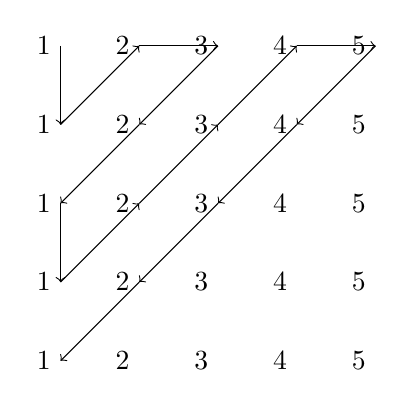
\begin{tikzpicture}
\draw[->] (0.5,-0.5) -- (0.5,-1.5);
\draw[->] (0.5,-2.5) -- (0.5,-3.5);
\draw[->] (1.5,-0.5) -- (2.5,-0.5);
\draw[->] (3.5,-0.5) -- (4.5,-0.5);

\draw[->] (0.5,-1.5) -- (1.5,-0.5);

\draw[->] (2.5,-0.5) -- (1.5,-1.5);
\draw[->] (1.5,-1.5) -- (0.5,-2.5);

\draw[->] (0.5,-3.5) -- (1.5,-2.5);
\draw[->] (1.5,-2.5) -- (2.5,-1.5);
\draw[->] (2.5,-1.5) -- (3.5,-0.5);

\draw[->] (4.5,-0.5) -- (3.5,-1.5);
\draw[->] (3.5,-1.5) -- (2.5,-2.5);
\draw[->] (2.5,-2.5) -- (1.5,-3.5);
\draw[->] (1.5,-3.5) -- (0.5,-4.5);

\node [left] at (0.5,-0.5) {1};
\node [left] at (0.5,-1.5) {1};
\node [left] at (0.5,-2.5) {1};
\node [left] at (0.5,-3.5) {1};
\node [left] at (0.5,-4.5) {1};
\node [left] at (1.5,-0.5) {2};
\node [left] at (1.5,-1.5) {2};
\node [left] at (1.5,-2.5) {2};
\node [left] at (1.5,-3.5) {2};
\node [left] at (1.5,-4.5) {2};
\node [left] at (2.5,-0.5) {3};
\node [left] at (2.5,-1.5) {3};
\node [left] at (2.5,-2.5) {3};
\node [left] at (2.5,-3.5) {3};
\node [left] at (2.5,-4.5) {3};
\node [left] at (3.5,-0.5) {4};
\node [left] at (3.5,-1.5) {4};
\node [left] at (3.5,-2.5) {4};
\node [left] at (3.5,-3.5) {4};
\node [left] at (3.5,-4.5) {4};
\node [left] at (4.5,-0.5) {5};
\node [left] at (4.5,-1.5) {5};
\node [left] at (4.5,-2.5) {5};
\node [left] at (4.5,-3.5) {5};
\node [left] at (4.5,-4.5) {5};


\end{tikzpicture}

趋向于极限1,2,3,。。。。

$\\$
$\{x_n\}趋向于(0,1)中任意有理数$

例

$\begin{matrix}
1 & \frac{1}{2} & \frac{1}{3} & \frac{1}{4} & ...  \\
\frac{1}{2} & \frac{2}{2} & \frac{3}{2} & \frac{4}{2} & ... \\
\frac{1}{3} & \frac{2}{3} & \frac{3}{3} & \frac{4}{3} & ... \\
\frac{1}{4} & \frac{2}{4} & \frac{3}{4} & \frac{4}{4} & ... \\
...
\end{matrix}$

$\\$
任意数列存在单调子列$\{x_{nk}\}$

$1^\circ 若\{x_n\}中无最大项,任取x_{n1},x_{n2},x_{n3},......构造法易知$

$2^\circ 若\{x_n\}中有最大项,记为x_{n1},后面取max\{x_{i>n1}\},记为x_{n2},易知构造法,若后续无最大项,则到情况1$

$3^\circ 以上,已构造出一个单调子列,由单调有界定理可知,若有界则有收敛子列$

$\nl$
例 设$$\{x_n\}有界,\sup_{n \in \bm N}\{x_n\}=\beta \notin \{x_n\}$$

求证$\{x_n\}$中有严格递增子列,$$设\lim_{n \to \infty}x_{nk}=\beta$$

$
证明:先令\varepsilon_1=1,由确界定义可知\exists x_{n1} \in \{x_n\}:\beta -1 < x_{n1} < \beta
$

$考虑集合S_1=\{x_n|n>n_1\}仍有sup S_1 = \beta$

$再令\varepsilon_2=min(\frac{1}{2},\beta-x_{n1})$

$必\exists x_{n2} \in S_1 \subset \{x_n\}: \beta- \varepsilon_2<x_{n2}<\beta (n_2>n_1)且x_{n2}>x_{n1}$

$一般的,记S_{k-1}=\{x_n|n>n_{k-1}\},令\varepsilon_k=min(\frac{1}{k},\beta-x_{nk-1}),必$

$\exists x_{nk} \in S_{k-1} \subset \{x_n\},\beta - \varepsilon_k < x_{nk} < \beta, n_k > n_{k-1},且x_{nk} > x_{nk-1} \forall k \in \bm N$

$$因为0<\varepsilon_k \le \frac{1}{k} 故\lim_{n \to \infty}\varepsilon = 0. 令k \to \infty 由迫敛性定理可得 \lim_{n \to \infty}x_{nk}=\beta$$

$且\{x_{nk}\}严格递增$

$\nl$
Ex:

$x_1=\frac{a}{2}, x_n=\frac{a}{2}-\frac{x_{n-1}^2}{2}  (0<a<1)$

解:$x_{2n-1}>x_{2n+1} ~~~~    x_{2n}<x_{2n+2}$

$x_{2n-1}>x_{2n} \ge x_2, x_{2n}<x_{2n+1}<x_1$

故奇偶子列分别收敛

$$\ntinf x_n = \ntinf (\frac{a}{2}-\frac{x_{n-1}^2}{2}),\ntinf x_{n+1} = \ntinf (\frac{a}{2}-\frac{x_{n}^2}{2})$$

$(\beta = \frac{a}{2}-\frac{\alpha ^2}{2}, \alpha = \frac{a}{2}-\frac{\beta ^2}{2}) \Rightarrow \alpha = \beta$

$\nl$
柯西定理见书P52-P53

柯西第二定理

Ex:$x_n = \frac{n^n}{n!}$

$\ntinf \frac {n}{\sqrt[n]{n!}}=\ntinf \frac{x_{n+1}}{x_n}=\ntinf (1+\frac{1}{n})^n=e$

Ex:$x_n=\sqrt[n]{\begin{matrix}\underbrace{ [a[a...[a]]] } \\ n \end{matrix}},n \in N$

证明$\{x_n\}$收敛

$\\$

$\nl$

$\S 函数的极限$


一、函数极限概念

(1)过程与极限

一.离散型

二.连续型

1$^\circ x \to + \infty $

2$^\circ x \to - \infty $

3$^\circ x \to \infty 双侧$

4$^\circ x \to x_0^- ,x<x_0$

5$^\circ x \to x_0^+ ,x>x_0 $

6$^\circ x \to x_0 $

$P64.P65 , 1^\circ ~3^\circ$

$P63,P55, 4^\circ ~ 6^\circ$

$\nl$
$当x \to x_0时,f(x)极限不存在$

$\forall A \in R, \exists \varepsilon_0>0, \forall \delta>0:|f(x_a)-A| \ge \varepsilon_0,\exists x_a \in U_0(x_0,\delta)$

$\forall A \in R, \exists \varepsilon_0>0, 及|x_n| (x_n \to x_0,x_n \ne x_0,n \in N),|f(x_n)-A| \ge \varepsilon_0,\forall n \in N$

$\nl$
$例:证明 \ntx{x_0}f(x)=A$

$|f(x)-A| \le ... < c·|x-x_0|,可令|x-x_0|<\delta ,利用......,取\delta =g(\varepsilon)或\delta = min(g(\varepsilon),c')c'为常数。$

则有$|f(x)-A|<\varepsilon,\forall x \in U_0(x_0,\delta)$

$\nl$

$函数在不同进程中极限之关系$

$①P64 ②\ntinf f(x) = A \Leftrightarrow \ntx{+\infty,-\infty} f(x) = A $

$③Heine定理 P59$
$\xtx{x_0}f(x)=A的充要条件是$

$\forall \{x_n\} (x_n \to x_0,x_n \ne x_0) \ntinf f(x_n)=A (可改为\{f(x_n)\}都存在)$

利用:充分性,判断函数极限之性质,必要性,函数极限存在

$\nl$
柯西收敛准则,见P104

$\xtx{x_0}f(x)存在充要条件$

$\forall \varepsilon>0,\exists \delta>0,\forall x',x'' \in U_0(x_0,\delta)有|f(x')-f(x'')|<\varepsilon$

$\\$
$c<b<a,|b|<|a|+|c|$

$\nl$
例:
$\xtx{0}(sinx+cosx)^{\frac{1}{x}}= \xtx{0}(1+sinx+cosx-1)^{\frac{1}{sinx+cosx-1}·\frac{sinx+cosx-1}{x}}$

$=e^{\xtx{0} \frac{sinx+cosx-1}{x}}=e^1=e$

$\xtx{0}\frac{ln(1+ax)}{x}=a,a=a\cdot ln(1+ax)^{\frac{1}{ax}} = \frac{ln(1+ax)}{x} < \frac{ln(1+x)^a}{x} = \frac{aln(1+x)}{x}=aln(1+x)^{\frac{1}{x}}$

$\xtx{0}\frac{e^{ax}-1}{x}=a$

$\xtx{0}\frac{a^x-1}{x}=lna$

$\\$
三、数量级及其应用

1)无穷小与无穷大

定义:$若\xtx{\Delta} f(x)=0,称f(x)为 x \to \Delta 时无穷小 P30$

$\Delta :(x_0,x_0^{\pm},\infty,\infty^{\pm})$

性质,在$x \to \Delta 的同一过程中$

(i)有限个无穷小之和在该过程中仍然无穷小

(ii)有界函数与无穷小乘积仍为无穷小

(iii)有限个无穷小乘积仍为无穷小

$\\$
P46 无穷大
性质P49,P67,P68

$\nl$
Ex:f(x)=x·sinx, $x \to + \infty 无界,但未必f(x) \to \infty$

$\nl$
高阶,P92

$\nl$
Ex:证明 $o(x^n)+o(x^m)=o(x^n)   (m \ge n)$

只需证
$\xtx{0} \frac{o(x^n)+o(x^m)}{x^n}=0$

$\xtx{0} \frac {o(x^n)}{x^n}=0$

$\xtx{0} \frac {o(x^m)}{x^m} \frac{x^m}{x^n} = 0·1 = 0$

$\nl$
无穷小之等价代换(P93)

$x \to 0 可作 \varphi(x) \to 0代换\varphi(x)=x$

$sinx~x~tgx ~~~ (基本)$

$arcsinx~arctgx~x(容易)$

$1-cosx ~ \frac{1}{2}x^2,\sqrt[n]{1+x}-1~\frac{x}{n}$

$ln(1+x)~x,e^x-1~x,a^x-1~xlna$

$\nl$
Ex.$f(x)在(0,+\infty)上有f(x^2)=f(x)$

且$\xtx{0+}f(x)=\xtx{+\infty}f(x)=f(1)$

$则f(x)=f(1) \forall x \in (0,+ \infty)$

$证明:当\forall x \in (0,1) f(x)=f(x^2)=....f(x^{2^n})$

$\ntx{\infty}x^{2^n}=0,用归结原理可知f(x)=\ntx{\infty}f(x^{2^n})=...=f(1)$

$当x\in (1,+\infty)类似可证$

$x \to \infty,(1-\frac{1}{x^2})^{x^2}=\frac{1}{(1+\frac{1}{-x^2})^{-x^2}}=\frac{1}{e}$

$x \to 0,\frac{a^{x^2}-b^{x^2}}{(a^x-b^x)^2}=\frac{1}{lna-lnb}$

$\nl$
$f(x)为三次多项式,且\xtx{2a}\frac{f(x)}{x-2a}=\xtx{4a}\frac{f(x)}{x-4a}=1,求\xtx{3a}\frac{f(x)}{x-3a}$

$设f(x)=b(x-2a)(x-4a)(x-c),代入上式可得$

$-2ab(2a-c)=1$

$2ab(4a-c)=1$


故有$a^2b=\frac{1}{2},c=3a$

$\xtx{3a}\frac{f(x)}{x-3a}=-\frac{1}{2}$


\end{document}

